\chapter{Analysis of the Impact of Heterogeneity Losses due to Upscaling in Well Testing Simulations}
\label{chapterResults}

Chapters \ref{mathematicalFormulation} to \ref{solution} show how the reservoir simulator utilized in this project has been developed and validated. Chapters \ref{upscaling} and \ref{wellTesting} show introductions of upscaling and well testing, the areas investigated by this project. This chapter shows the analysis of the effects of upscaling in well testing simulations, the main application of the simulator developed in this project. Several models have been created and put under flow simulation. The results of bottom hole pressure, pressure drop, and Bourdet derivative have been plotted and compared. The idea is to visualize how a numerical model for a pressure transient analysis would provide different results for a fine grid versus an upscaled one. The first section of this chapter shows the details of the construction of each of those models and the parameters of the simulation. The last section will show the results obtained in the simulation and its analyzes.

\section{Models}

Eight different cases have been created and simulated for outputting bottom hole pressure, pressure drop, and the Bourdet derivative. They are parallelepipedal models of synthetic sandstone reservoirs. Table \ref{table10.1} shows the common characteristics for all the cases. The fluid model for all the scenarios is the same as utilized in the validation cases and is illustrated by Figure \ref{fig:30}. The porosity-permeability relationship is equal for all the models and follows the correlation illustrated in Figure \ref{fig:35} and in the Eq. \ref{results1}.
\begin{table}[htbp]
	\centering
	\caption{Common characteristics for all the simulation cases.}
	\begin{tabular}{c c}
	\toprule
	Parameter & Value (if applicable)\\
	\midrule
	Reservoir length in the $x$ direction & 2559.03 ft\\
	Reservoir length in the $y$ direction & 2559.03 ft\\
	Reservoir length in the $z$ direction & 164.04 ft\\
	Boundary conditions & Sealed reservoir \\
	Well & Vertical well in the\\
	& center of the reservoir\\
	Completions & From the top to the\\
	& bottom of the reservoir\\
	Average porosity & 20\%\\
	Average horizontal permeability & 51.59 mD\\
	Average vertical permeability & 51.59 mD\\
	Formation compressibility & $1.31 x 10^{-4}$ psi$^{-1}$\\
	Fluid compressibility &  1.41 x 10$^{-5}$ psi$^{-1}$\\
	Depth of the topmost layer & 10,498.69 ft\\
	Reference depth for the initial pressure & 10,498.69 ft\\
	Initial pressure at the reference depth & 3,916.01 psi\\
	Well radius & 6 in\\
	Skin factor & -0.5\\
	\bottomrule
\end{tabular}
	\label{table10.1}
\end{table}
\begin{figure}[H]
	\centering
	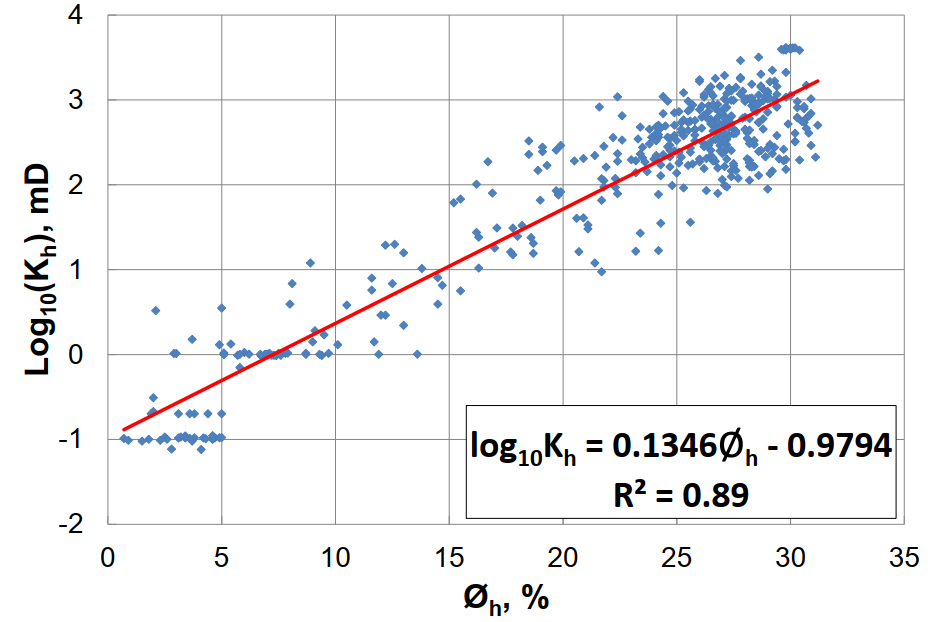
\includegraphics[width=0.8\linewidth]{Images/35}
	\caption{Relationship between the porosity and permeability of the UNISIM-I, a synthetic sandstone model based on the Namorado Field, Campos Basin of Brazil. Source: \cite{Avansi2015}. The eight models constructed in this chapter have the same porosity-permeability relationship as shown in this picture.}
	\label{fig:35}
\end{figure}
\begin{equation}\label{results1}
k_h = 10^{(0.1346\phi)-0.9794}.
\end{equation}
In other words, Table \ref{table10.1}, Figure \ref{fig:30}, Figure \ref{fig:35} and Eq. \ref{results1} shows the common characteristics shared between the eight models. What differs one case to another is the size and number of the grid blocks and the standard deviation of the porosity and permeability. 

Scenarios 1 and 2 are homogeneous in terms of porosity and permeability. While scenario 1 has a fine grid, scenario two has a coarse grid constructed by the upscaling of scenario 1. In other words, scenario 2 is the upscaled version of scenario 1. Each direction of scenario 2 presents half the number of grid blocks in comparison to scenario 1. Since scenario 1 is homogeneous, there is no spatial variation of porosity and permeability and scaling up can be done straightforwardly, without the need for averaging techniques.

Scenario 3 has heterogeneous permeabilities and porosities. The porosity is populated by utilizing a normal distribution with a mean equals to 20\%, the same as scenario 1, and a standard deviation equals 3\%. Then, the horizontal permeabilities are calculated by utilizing the correlation shown in Eq. \ref{results1}. Finally, the vertical permeabilities are set to be equals to 10\% of the horizontal for each grid bock. Thus, both the horizontal and vertical permeabilities follow log-normal distributions with the same means as in scenario 1. Scenario 4 is the upscaled version of scenario 3. Since porosity and permeability are not homogeneous, it is necessary to perform an upscaling technique. A simple volumetric averaging has been utilized for upscaling the porosity, as shown in Eq. \ref{Upscaling3}. Then, an arithmetic-harmonic averaging has been utilized for scaling up the permeability tensor as demonstrated by Eq. \ref{arithmeticharmonic}.  

Scenario 5 is essentially the same as scenario 3, with the difference that the standard deviation of the porosity is set to be equal to 6\%, the double of the one from scenario 3. That would result in permeabilities with higher standard deviations as well since they are populated by following the same rules as in scenario 3. Scenario 6 is scenario 5 upscaled by the same approach described above.

Scenario 7 is scenario 3 with a standard deviation of porosity set to be equals to 1.5\%, half of the one from scenario 3. Again, the permeabilities have been populated in the same way as described above. Finally, the last scenario, 8, is the upscaled version of scenario 7. Table \ref{fig:36} summarizes the differences between each model:

\begin{table}[htbp]
	\centering
	\caption{Diference between each simulation scenario.}
	\label{fig:36}
	\begin{tabular}{c c c c c c c}
		\toprule
		Case & Nx & Ny & Nz & Upscaling & Heterogeneity & $\phi$ Standard Deviation\\
		\midrule
		1 & 26 & 26 & 20 & No & Homogeneous & 0\\
		2 & 13 & 13 & 10 & No & Homogeneous & 0\\
		3 & 26 & 26 & 20 & Yes & Heterogeneous & 3\%\\
		4 & 13 & 13 & 10 & Yes & Heterogeneous & 6\%\\
		5 & 26 & 26 & 20 & Yes & Heterogeneous & 6\%\\
		6 & 13 & 13 & 10 & Yes & Heterogeneous & 6\%\\
		7 & 26 & 26 & 20 & Yes & Heterogeneous & 1.5\%\\
		8 & 13 & 13 & 10 & Yes & Heterogeneous & 1.5\%\\
		\bottomrule
	\end{tabular}
\end{table}

Appendix \ref{appendixModelsDescriptions} shows in more detail the porosity-permeability distributions of scenarios 3 to 8. The next section shows the results obtained by the simulation done in those models.

\section{Results}

%Scenario 4 is the coarsened version of scenario 3. An arithmetic-harmonic averaging technique has been utilized for scaling up the permeability tensor as shown in the Eq. . For upscaling the porosity, a simple volumetric averaging technique has been utilized, as seen in the Eq. \ref{Upscaling3}. 

%The Figures \ref{fig:37} to \ref{fig:39} show the porosity and permeability distributions for both the case 3 and case 4.

%\begin{figure}[H]
%	\centering
%	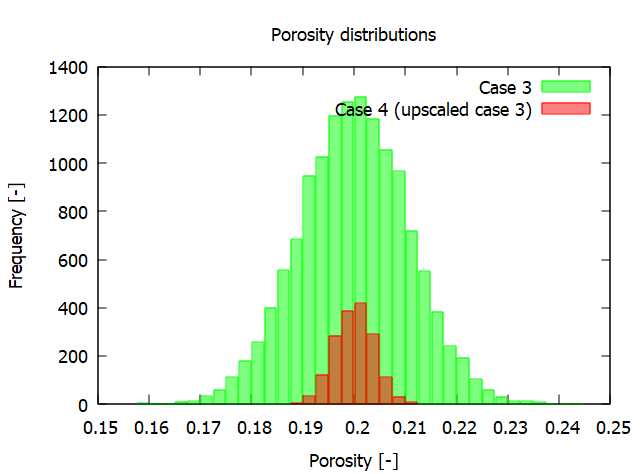
\includegraphics[width=0.8\linewidth]{Images/37}
%	\caption{Porosity distribution for case 3 and its upscaled version (case 4).}
%	\label{fig:37}
%\end{figure}
%
%\begin{figure}[H]
%	\centering
%	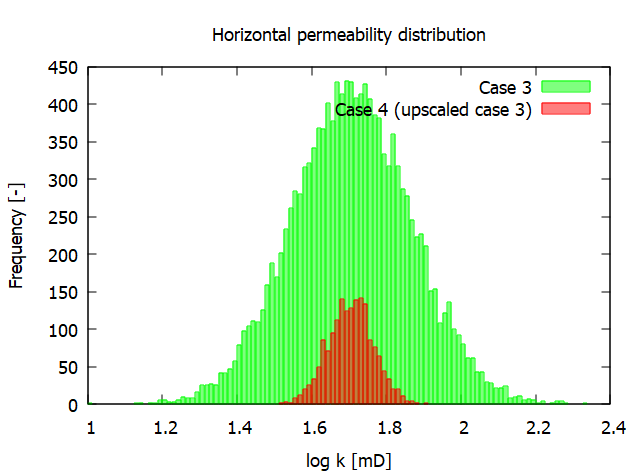
\includegraphics[width=0.8\linewidth]{Images/38}
%	\caption{Horizontal permeability distribution for case 3 and its upscaled version (case 4).}
%	\label{fig:38}
%\end{figure}
%
%\begin{figure}[H]
%	\centering
%	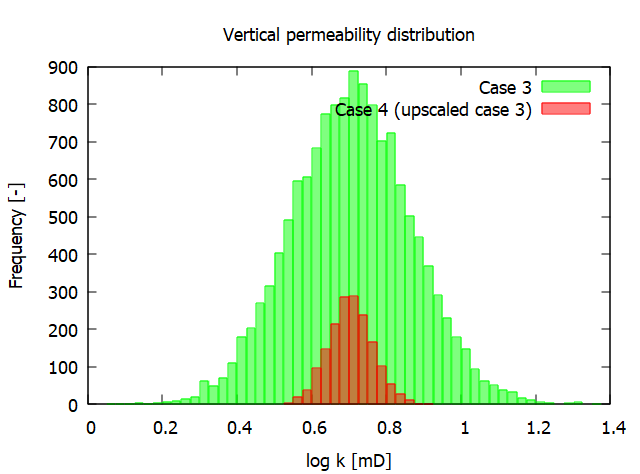
\includegraphics[width=0.8\linewidth]{Images/39}
%	\caption{Vertical permeability distribution for case 3 and its upscaled version (case 4).}
%	\label{fig:39}
%\end{figure}
%Figures \ref{fig:37} to \ref{fig:39} display the petrophysical distributions for both the fine grid and its upscaled model. One could see that the red histograms' columns (upscaled model) are smaller than the green ones (fine model), that happens because the number of grid blocks for the coarse model is eight times less than in the fine one. Since the vertical axis displays the frequency in absolute terms, the upscaled model has naturally smaller columns. Another difference between the red and green is the dispersion: the standard deviation of the fine model is superior to the one of the upscaled version. That is a natural characteristic of the upscaling: the grid blocks were averaged implying in a lower dispersion in the coarse model. Figures \ref{fig:42} to \ref{fig:44} show the distribution of the other cases.

The previous section display the details of the eight models constructed for this study. All those cases have been put under flow simulation for a drawdown test scenario. The well is initially closed, and opens at the time of 0.1 day with a constant flow rate. Then, the simulation continues until the time is equal to 2 days. 

All those cases have been put under flow simulations for a drawdown test scenario, in which the well is set to be initially closed and opens at the time 0.1 day, with the simulation ending at the time of 2 days. Figures \ref{fig:47} to \ref{fig:48} display the outputs of bottom hole pressure for the simulations. Figures \ref{fig:51} to \ref{fig:55} shows the log-log diagnostic plot for this drawdown test, comprising the pressure drop and Bourdet derivative curves for each case. 

Figure \ref{fig:46} shows the BHP for all the fine models. One could see that the results for the homogeneous model (case 1) were very similar to the ones of the model with a lower standard deviation (case 7). The BHP for case 5 (higher standard deviation) was considerably higher than the ones for the cases with lower dispersions.

%\begin{figure}[H]
%	\centering
%	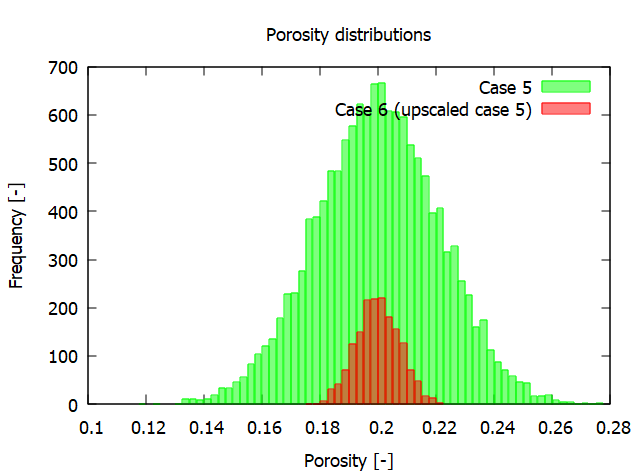
\includegraphics[width=0.8\linewidth]{Images/42}
%	\caption{Porosity distribution for case 5 and its upscaled version (case 6).}
%	\label{fig:42}
%\end{figure}
%
%\begin{figure}[H]
%	\centering
%	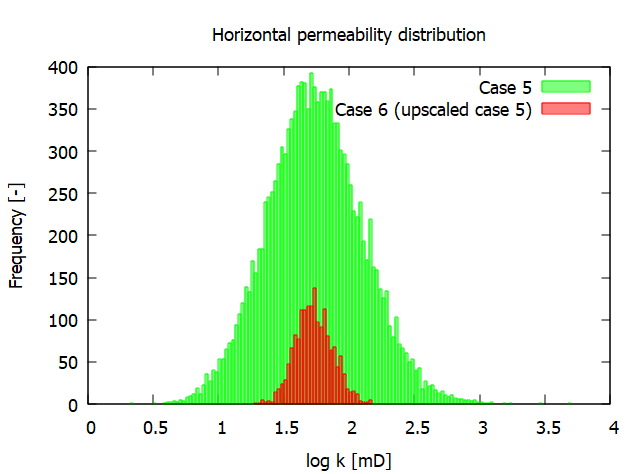
\includegraphics[width=0.8\linewidth]{Images/41}
%	\caption{Horizontal permeability distribution for case 5 and its upscaled version (case 6).}
%	\label{fig:41}
%\end{figure}
%
%\begin{figure}[H]
%	\centering
%	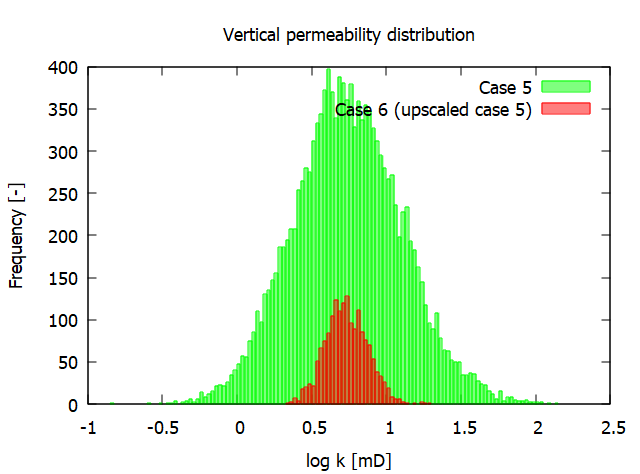
\includegraphics[width=0.8\linewidth]{Images/40}
%	\caption{Vertical permeability distribution for case 5 and its upscaled version (case 6).}
%	\label{fig:40}
%\end{figure}
%
%\begin{figure}[H]
%	\centering
%	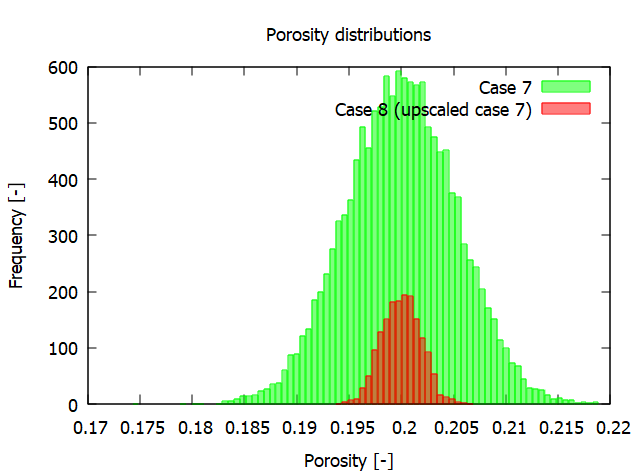
\includegraphics[width=0.8\linewidth]{Images/43}
%	\caption{Porosity distribution for case 7 and its upscaled version (case 8).}
%	\label{fig:43}
%\end{figure}
%
%\begin{figure}[H]
%	\centering
%	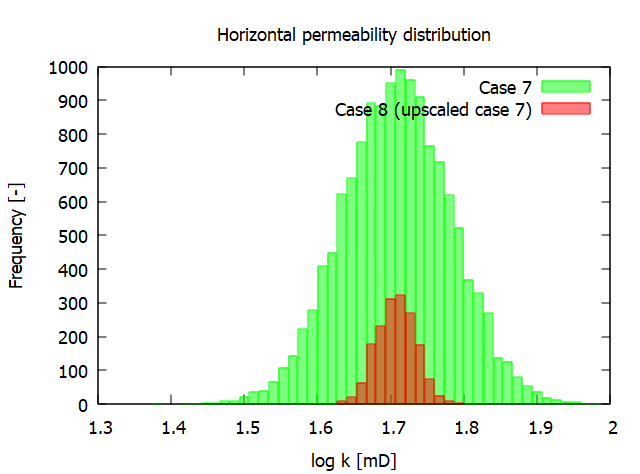
\includegraphics[width=0.8\linewidth]{Images/45}
%	\caption{Horizontal permeability distribution for case 7 and its upscaled version (case 8).}
%	\label{fig:45}
%\end{figure}
%
%\begin{figure}[H]
%	\centering
%	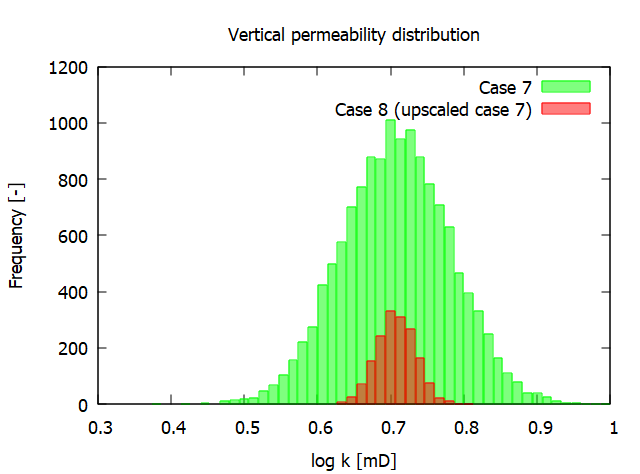
\includegraphics[width=0.8\linewidth]{Images/44}
%	\caption{Vertical permeability distribution for case 7 and its upscaled version (case 8).}
%	\label{fig:44}
%\end{figure}

\begin{figure}[H]
	\centering
	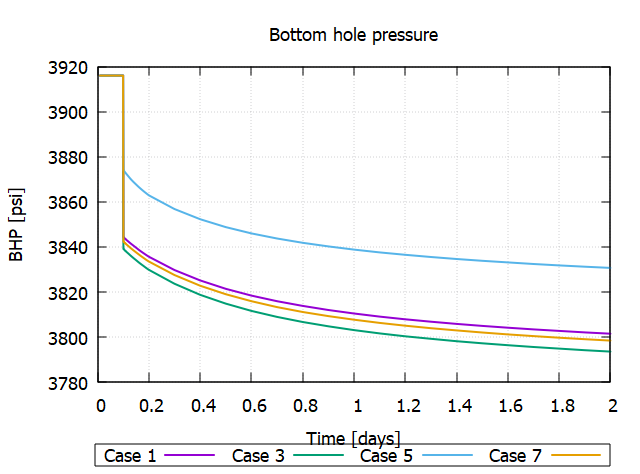
\includegraphics[width=0.8\linewidth]{Images/46}
	\caption{Bottom hole pressure for the fine models (case 1, case 3, case 5 and case 7).}
	\label{fig:46}
\end{figure}

\begin{figure}[H]
	\centering
	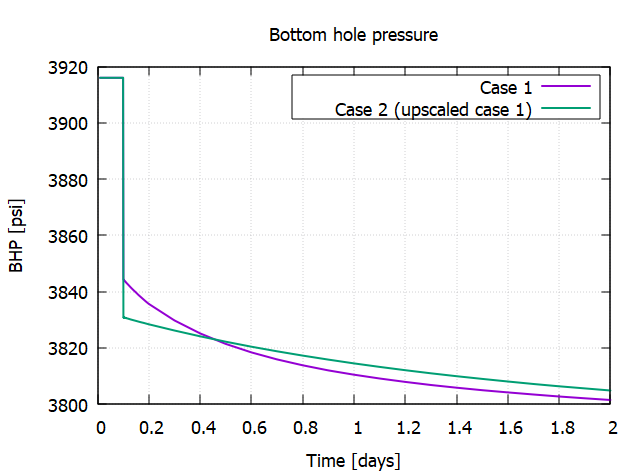
\includegraphics[width=0.8\linewidth]{Images/47}
	\caption{Bottom hole pressure for case 1 and its upscaled version, case 2.}
	\label{fig:47}
\end{figure}

\begin{figure}[H]
	\centering
	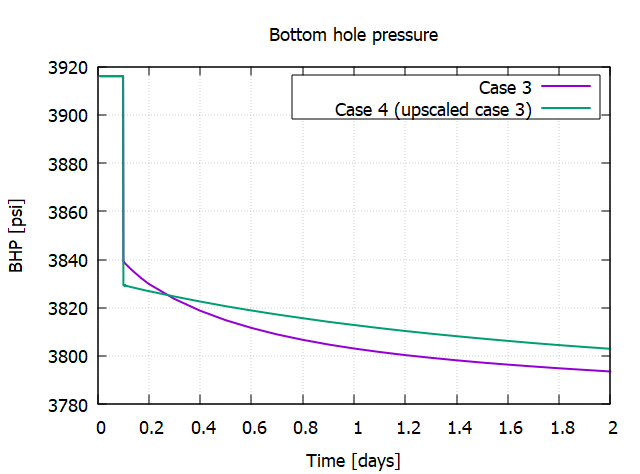
\includegraphics[width=0.8\linewidth]{Images/48}
	\caption{Bottom hole pressure for case 3 and its upscaled version, case 4.}
	\label{fig:48}
\end{figure}

Figure \ref{fig:47} shows the BHP for case 1 and case 2 (the upscaled version of case 1). One could see that the results are quite similar for each case, as expected since both cases present homogeneous porosity and permeabilities. Figure \ref{fig:48} shows similar results but for cases 3 and 4, homogeneous reservoirs. The difference between the curves is higher in those scenarios than in case 1 and 2. Nevertheless, this difference is still small, showing that the arithmetic-averaging upscaling represents the fine model with fairly good accuracy. Figures \ref{fig:49} to \ref{fig:50} display the same information for the cases 5 to 8. By looking at Figures \ref{fig:47} to \ref{fig:50}, one could see that the difference between coarse and fine models is consistently greater with higher standard deviations in the porosity and permeability distributions. 

Figure \ref{fig:51} shows the diagnostic log-log plot with the pressure drop and the Bourdet derivative for the cases 1 to 7. Case 1, 3, and 7 have very similar results. Case 5 present lower pressure drops and higher Bourdet derivatives than the other scenarios, as a consequence of its higher standard deviation. Figures \ref{fig:52} to \ref{fig:52} shows the diagnostic plot for each fine-coarse pair. Again, higher standard deviations are related to higher differences between fine and coarse curves. The Bourdet derivative is consistently lower for the coarse models in comparison with their fine pairs. Lower Bourdet derivatives are related to higher transmissibilities in the region near the wellbore. That could be one characteristic of the coarse models. 

\begin{figure}[H]
	\centering
	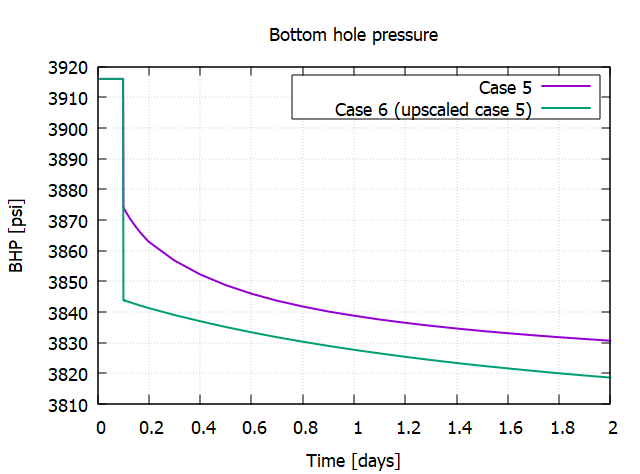
\includegraphics[width=0.8\linewidth]{Images/49}
	\caption{Bottom hole pressure for case 5 and its upscaled version, case 6.}
	\label{fig:49}
\end{figure}

\begin{figure}[H]
	\centering
	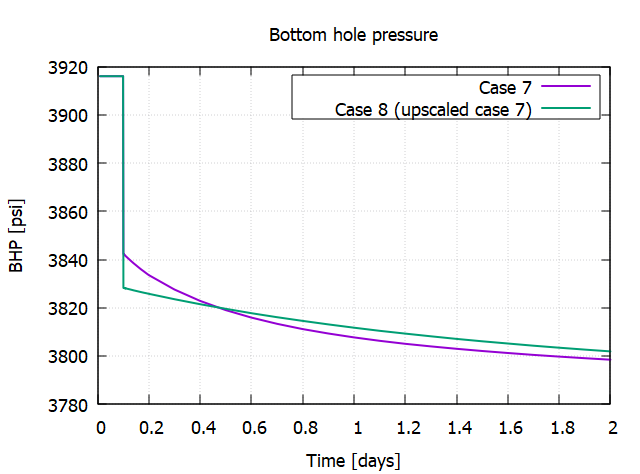
\includegraphics[width=0.8\linewidth]{Images/50}
	\caption{Bottom hole pressure for case 7 and its upscaled version, case 8.}
	\label{fig:50}
\end{figure}

\begin{figure}[H]
	\centering
	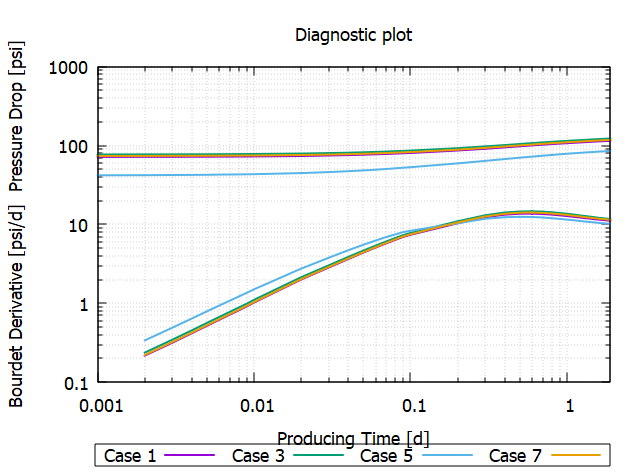
\includegraphics[width=0.8\linewidth]{Images/51}
	\caption{Pressure drop and Bourdet derivative for the fine models (case 1, case 3, case 5 and case 7).}
	\label{fig:51}
\end{figure}

\begin{figure}[H]
	\centering
	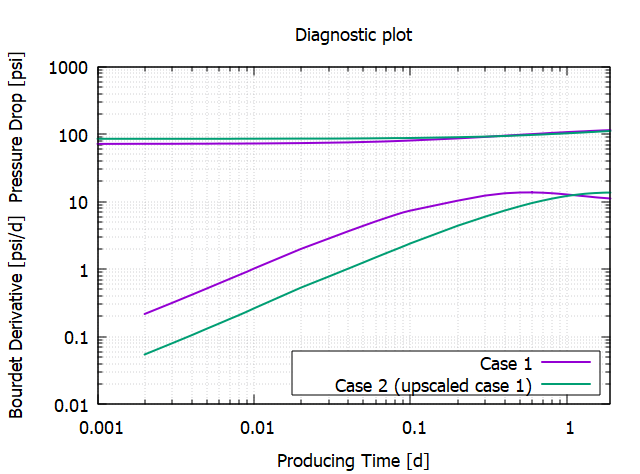
\includegraphics[width=0.8\linewidth]{Images/52}
	\caption{Pressure drop and Bourdet derivative for case 1 and its upscaled version, case 2.}
	\label{fig:52}
\end{figure}

\begin{figure}[H]
	\centering
	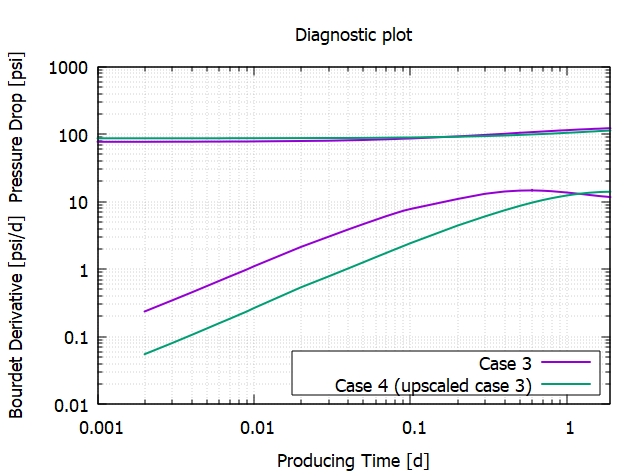
\includegraphics[width=0.8\linewidth]{Images/53}
	\caption{Pressure drop and Bourdet derivative the case 3 and its upscaled version, case 4.}
	\label{fig:53}
\end{figure}

\begin{figure}[H]
	\centering
	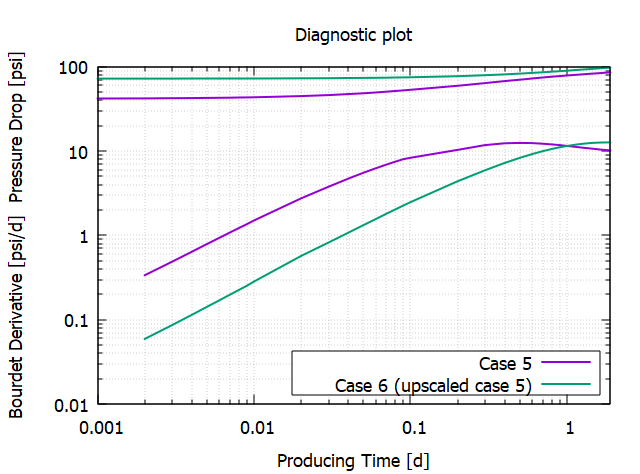
\includegraphics[width=0.8\linewidth]{Images/54}
	\caption{Pressure drop and Bourdet derivative the case 5 and its upscaled version, case 6.}
	\label{fig:54}
\end{figure}

\begin{figure}[H]
	\centering
	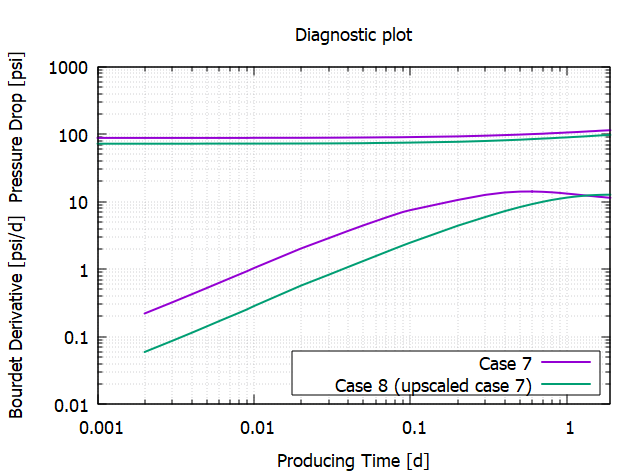
\includegraphics[width=0.8\linewidth]{Images/55}
	\caption{Pressure drop and Bourdet derivative the case 7 and its upscaled version, case 8.}
	\label{fig:55}
\end{figure}

